The application has three main components: a server for training and prediction, an Amazon S3 image storage server, and the client-side mobile application on iOS. 

\subsection{Pipeline}
Our pipeline starts in the mobile application. A user opens our application and takes a picture of a building they want to identify. The application sends the image to our server which processes the image, extracts features, and runs it against our classifier. The classifier will respond to the application with the a list of buildings it believes the image contains in order of highest confidence. The user is then presented the results alongside images of the building to help the user confirm their answer. When the user clicks the result, they are shown information about that landmark along with a position of where they are on a map. At the same time, a message is sent from the application to the server letting the server know what the real answer was. The motivation behind having users confirm the results of our classifier is that it lets our dataset grow as more users take pictures and read about the landmarks on Columbia's campus.

\begin{figure}
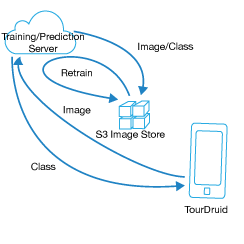
\includegraphics[width=86mm]{app_arch.png}

\caption{Application Architecture Diagram}
\label{overflow}

\end{figure}

\subsection{Server}
The server is built using Node.js and runs on linux machines. The server currently has two POST endpoints named \textit{/classify} and \textit{/confirm} that are reached by our mobile application. All communication between the client-side application and the server is in JSON. For every request sent to the \textit{/classify} endpoint, the server generates a unique ID that it returns to the client (along with the classifier's results). This ID is used to identify confirmation requests sent to the \textit{/confirm} endpoint, allowing our server to handle multiple classifications at once. When the server builds the classifier, it writes the codebook and TF-IDF matrix into files so the classifier avoids rebuilding those data structures for every request.

\subsection{Image Storage}

\subsection{Mobile Application}
